\documentclass[12pt,a4paper]{article}
\usepackage{graphicx}
\usepackage{url}
\usepackage{listings}
\usepackage{float}
\usepackage{afterpage}
 
\begin{document}
		\afterpage{\null\newpage}
		\newpage
	
	\begin{titlepage}
		\centering
		
\includegraphics[width=0.8\textwidth]{imagenes/logo_ugr.jpg}\par\vspace{1cm}
		{\scshape\LARGE Universidad de Granada \par}
		\vspace{1cm}
		{\scshape\Large Proyecto fin de Doble Grado en Ingenier\'ia Inform\'atica y Matem\'aticas\par}
		\vspace{1.5cm}
		{\huge\bfseries Una estrategia para bolsa basada en algoritmos evolutivos y su implementaci\'on en una plataforma de trading\par}
		\vspace{0.2cm}
		\noindent\rule{\textwidth}{1pt}
		\vspace{2cm}
		{\Large\itshape Miguel \'Angel Torres L\'opez\par}
		\vfill
		supervisado por\par
		{\large Prof. Jose Manuel Zurita L\'opez}
		
		\vfill
		
		% Bottom of the page
		{\large \today\par}
			
	\end{titlepage}
	
	\afterpage{\null\newpage}
	\newpage
	
	\tableofcontents
	
	\newpage
	
	\section{Fundamentos de Bolsa}
	
		\subsection{Mercado de valores}
		
		El mercado de valores o bolsa, es un tipo de mercado en el que se compran y venden productos burs\'atiles. Para este trabajo, prestaremos principal atenci\'on a las acciones, el producto burs\'atil m\'as simple de un mercado de valores.
		
		Una acci\'on corresponde con una pequeña participaci\'on en la empresa a la que pertenezca la acci\'on. De esta forma, inversores privados tiene la posibilidad de comprar porciones de empresas. Por ejemplo, si una empresa est\'a dividida en 200 acciones, tras comprar 50 de estas, ser\'iamos propietarios de una cuarta parte de la empresa. Esto puede reportarnos beneficios de distinta \'indole seg\'un las normas de la empresa. En ocasiones algunas empresas deciden repartir una determinada cantidad de dinero entre sus accionistas en relaci\'on a las ganancias obtenidas en un periodo (dividendo). Otras veces, ser poseedor de una gran parte de la empresa nos otorgar\'a derechos dentro de la misma, como por ejemplo participar en las decisiones importantes que se tomen.
		
		El mercado de valores espa\~nol abre de 9:00 a 17:30 de lunes a viernes. Cabe destacar que hay una aleatoriedad de 30 segundos y que, además, despu\'es del cierre hay un periodo de subasta de 5 minutos para evitar manipulaciones de los precios. No vamos a entrar en como funciona este sistema.
		
		\subsection{El valor de las acciones}
		
		El valor de una acci\'on no es fijo, va cambiando seg\'un la oferta y la demanda de las acciones de la empresa. Esto convierte a las acciones en un producto muy conveniente para especular.
		
		El mecanismo de compra y venta es el que define el valor de una acci\'on. Para comprar o vender, un inversor debe enviar a bolsa una orden de compra o venta, respectivamente. Tras enviar la orden, esta queda registrada y ser\'a ejecutada cuando sea posible. Aclaremos esto con un ejemplo sencillo:\\
		
		Supongamos que existe una empresa que tiene en el mercado cuatro acciones. Cada una de ellas pertenece a un propietario distinto, llam\'emosles A, B, C y D. 
		
		A tiene una orden de venta de su acci\'on a 4 euros y C tiene una orden de compra de una acci\'on a 1 euro. En esta situaci\'on ninguno puede vender ni comprar y el precio est\'a situado en 4 euros por acci\'on. Ahora bien, B decide vender su acci\'on por 3 euros. En el momento en el que realiza una orden de venta, el precio de las acciones baja a 3 euros. Esto no quiere decir que A venda su acci\'on a este precio. Para bajar de 4 a 3 euros deber\'ia cancelar la orden y realizar una nueva. En esta situaci\'on no se puede ejecutar ninguna orden en el mercado, como se puede ver en la figura \ref{fig:ordenes_ejemplo}.
		
				\begin{figure}[H]
					\centering
					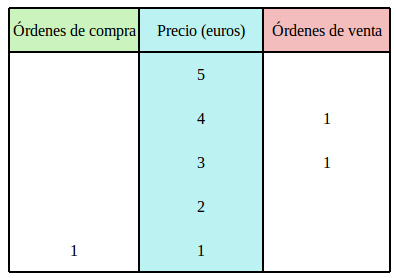
\includegraphics[scale=2]{imagenes/ordenes_ejemplo.png}
					\caption{Situaci\'on de las ordenes}
					\label{fig:ordenes_ejemplo}
				\end{figure}
		
		
		Tras ver que el precio de la acci\'on a bajado de 4 a 3 euros, el inversor D decide comprar y sit\'ua una orden de compra a 3 euros de una acciones. Entonces, la orden de venta de C y la orden de compra de D pueden ejecutarse. Ahora D pasa a tener 2 acciones y el mercado se queda con las dos \'ordenes de A y B, provocando que el precio de la acci\'on vuelva a subir a 4 euros.\\
		
		Adem\'as de las \'ordenes vistas en el ejemplo, existen otras un poco m\'as complejas:
		\begin{itemize}
			
			\item \textbf{Orden de mercado.} Se compran todas las acciones que se emitan en la orden al mejor precio posible. En caso de compra a los precios m\'as bajos, en caso de venta a los precios m\'as altos. Si B hubiera emitido una orden de mercado de una acci\'on, habría comprado la acci\'on de A a 4 euros.
			
			\item \textbf{Orden limitada.} Se compran todas las acciones que se emitan en la orden siempre y cuando su precio est\'e situado en el l\'imite establecido. Si D hubiera emitido una orden limitada a 3 euros de dos acciones, hubiera comprado por 3 euros la acci\'on de C pero no la de A, que est\'a a 4 euros. La orden permanece vigente hasta que la suma de las acciones sea comprada.
			
			\item \textbf{Orden on Stop.} No se hace efectiva hasta que el precio de las acciones llega al precio de la orden. En ese momento, la orden se convierte en una orden de mercado.
			
			\item \textbf{Orden Stop-Limit.} Este tipo de orden no se hace efectiva hasta que el precio de las acciones llega al precio de la orden. En ese momento, la orden se convierte en una orden limitada. Es muy frecuente que las plataformas ofrezcan este tipo de orden, pues funciona como seguro para no perder todo el capital cuando las acciones caen de precio r\'apidamente y el inversor posee acciones de la empresa. 
			
		\end{itemize} 
		
		\subsection{Corredores de bolsa o brokers}
	
		Para agilizar las transacciones en bolsa, no se permite que particulares env\'ien \'ordenes al mercado. Esta tarea se delega en los corredores de bolsa o \textit{brokers}. La entidad de \textit{broker} se encarga de captar inversores, colocar \'ordenes y presentar a compradores con vendedores. Para ser broker se debe aprobar un examen y demostrar que se tienen los conocimientos necesarios. Por este trabajo se lleva una comisi\'on que todo inversor debe abonar. 
		
		Las comisiones pueden ser de dos tipos:
		
		\begin{itemize}
			\item \textbf{Comisiones fijas.} Son un valor fijo que cada broker cobra. Puede ser por transacci\'on y por tiempo de servicio. Las comisiones fijas son beneficiosas para inversores con un gran capital.
			
			\item \textbf{Comisiones variables.} Son precios variables que dependen del país de inversión, la cantidad invertida e incluso el tiempo. Las comisiones variables afectan en misma medida a inversores grandes y peque\~nos.
		\end{itemize}
		
		La mayor\'ia de los corredores de bolsa tienen comisiones mixtas. No corresponde a este trabajo discutir m\'as all\'a sobre este tema. De ahora en adelante asumiremos unas comisiones variables. 
	
	\newpage
	\section{Plataformas de Trading}		
	
		\subsection{MetaTrader5}
		
    	Podemos observar que es una plataforma ampliamente usada, por tanto es f\'acil encontrar ejemplos iniciales o ayuda t\'ecnica. Se nos oferta en la p\'agina web de la plataforma\cite{metatraderweb} una demo gratuita con acceso a casi todos los recursos. 
		
		La programaci\'on de las estrategias se divide en varios archivos con unas especificaciones concretas. No obstante, existe una tienda empotrada en la plataforma para comprar y vender estrategias, \'indices o bibliotecas con otros usuarios. Cada producto est\'a puntuada por los usuarios que la han usado.\\
		
		A pesar de todas estas ventajas, no usaramos MetaTrader5 por ser de car\'acter privativo. Adem\'as, el lenguaje de programaci\'on de las estrategias es MQL5, un lenguaje propio de la plataforma que nos impide usar con facilidad bibliotecas externas.
	
		\subsection{Backtrader}
		
		Backtrader es un framework de libre licencia realizado en el lenguaje Python. La p\'agina web de la plataforma\cite{backtraderweb} contiene una amplia documentaci\'on en la que se explican todos los componentes del framework. Asimismo encontramos el m\'etodo de instalaci\'on y un tutorial de iniciaci\'on.
		
		El framework viene con indicadores ya programados, aunque te permite hacer m\'as de forma manual. Para producir gr\'aficos hay que instalar una librer\'ia adicional, esto no es problema porque viene integrado en la instalaci\'on como veremos.\\
		
		
		\subsubsection{Instalaci\'on}
		
		Pasamos ahora a su instalaci\'on. Necesitamos tener la versi\'on 2.7 de Python, tal y como se indica en la documentaci\'on de backtrader\cite{backtraderdoc} que podemos encontrar en su p\'agina web. Para comprobar la versi\'on podemos usar el comando \textit{python -Version}. En caso de no tener instalado Python o no tener la versi\'on indicada, podemos instalarlo usando \textit{sudo apt-get install python2.7}.\\
		
		El framework backtrader est\'a disponible, desde el c\'odigo fuente en Github. No obstante, tambi\'en esta disponible para el instalador de paquetes de Python pip. Si no est\'a instalado pip, podemos hacerlo con el comando \textit{sudo apt-get install python-pip}.\\
		
		Una vez llegados a este punto, podemos optar por una versi\'on con posiblidad de generar gr\'aficas o no. Para facilitar el an\'alisis de resultados, instalaremos la versi\'on con plotting con el comando \textit{pip install backtrader[plotting]} como podemos ver en la figura \ref{fig:pip_backtrader}. El mismo comando quitando la directiva \textit{[plotting]} instala la versi\'on sin gr\'aficas.\\
		
		\begin{figure}[H]
			\centering
			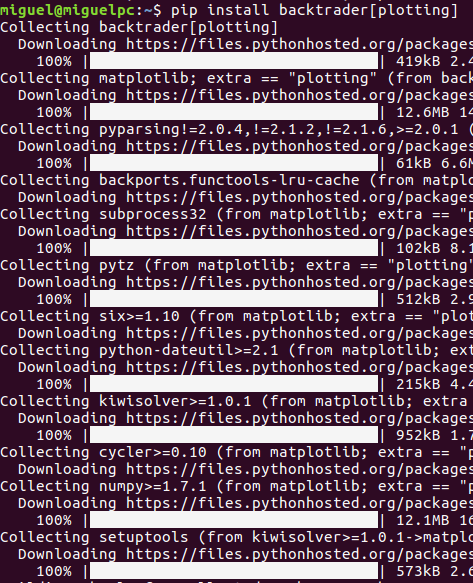
\includegraphics[scale=0.4]{imagenes/pip_backtrader.png}
			\caption{Resultado de instalar backtrader con plotting}
			\label{fig:pip_backtrader}
		\end{figure}
		
		Observamos que se han instalado otros paquetes adicionales. En concreto se ha instalado el paquete numpy, que m\'as tarde nos ser\'a \'util como herramienta matem\'atica.
		
		
		\subsubsection{Preparaci\'on del entorno}
		
		Una de las estructuras de datos m\'as comunes en backtrader son las l\'ineas. Una l\'inea no es m\'as que un conjunto de pares ordenados por uno de los elementos de menor a mayor. Por ejemplo, al hablar de un valor de mercado tenemos 5 l\'ineas: valor de apertura, valor de salida, valor m\'aximo, valor m\'inimo y volumen de compra/venta. 
		
		Al acceder a cada l\'inea hay que tener en cuenta que no usa la indexaci\'on de un vector en un lenguaje com\'un. En su lugar, el \'indice 0 representa el instante actual y para acceder a instantes anteriores usaremos \'indices negativos, por ejemplo:
		
		\begin{lstlisting}[basicstyle=\tiny]
	self.sma = SimpleMovingAverage(...)
	valor_actual            = self.sma[0]
	valor_instante_anterior = self.sma[-1]
		\end{lstlisting}
		
		\vspace{0.8cm}
		
		Antes de ver como crear una estrategia, vamos a ver como podemos simular una prueba introduciendo unos datos y un presupuesto inicial. Para ello, en un archivo con formato py para que podamos ejecutar con Python escribimos el siguiente c\'odigo:
		
		\begin{lstlisting}[basicstyle=\tiny]
from __future__ import (absolute_import, division, print_function, unicode_literals)
		
import datetime
import os.path
import sys
import backtrader as bt # Importar todas las herramientas de backtrader
		
if __name__ == '__main__':
	cerebro = bt.Cerebro()
		
# Crear un paquete de datos
	data = bt.feeds.YahooFinanceCSVData(
	dataname='YAHOO',  # Ruta absoluta donde se encuentran los datos descargados de YAHOO! Finance
# Fecha inicial de los datos
	fromdate=datetime.datetime(2000, 1, 1),
# Fecha final de los datos
	todate=datetime.datetime(2000, 12, 31),
	reverse=False)
		
# Activar los datos en el cerebro
	cerebro.adddata(data)
# Establecer dinero inicial    
	cerebro.broker.setcash(100000.0)
		
	print('Starting Portfolio Value: %.2f' % cerebro.broker.getvalue())
	cerebro.run()   # EJECUTAR BACKTESTING (AHORA MISMO, SIN NINGUNA ESTRATEGIA)
	print('Final Portfolio Value: %.2f' % cerebro.broker.getvalue())
		\end{lstlisting}
		
		\vspace{0.5cm}
		
		Notemos que se trata de una archivo Python en el que solo hemos tenido que importar el paquete \textit{backtrader}. Por tanto, en el caso de necesitar otros paquetes para realizar nuestra estrategia, solo tenemos que incorporarlos de forma habitual.\\
		
		En este ejemplo, no le hemos especificado a la clase \textit{cerebro} cu\'al va a ser la estrategia a seguir. Por este motivo, al hacer la simulaci\'on el presupuesto inicial y final no var\'ian. Para ejecutar el backtesting simplemente se ejecuta el script de Python con el comando \textit{python rutadelscript.py} en terminal. Nos dar\'a un fallo, la ruta donde deber\'ia estar el fichero con los datos est\'a vac\'ia, pues no hemos descargado ning\'un archivo de datos. Este tema se abordar\'a en la secci\'on \ref{sec:get_data}.
		
		
		\subsubsection{La primera estrategia}
		
		Antes de programar la primera estrategia de \textit{trading}, vamos a ilustrar con una estrategia f\'util c\'omo estructurar una clase para que backtrader pueda trabajar con ella como tal. La estructura b\'ascia es una clase con un m\'etodo \textit{\_\_init\_\_} y otro m\'etodo llamado \textit{next}. 
		
		El primero puede usarse para instanciar y agrupar los datos que requiere nuestra estrategia. El segundo m\'etodo es llamado en cada instante por backtrader. Consideramos que un instante es cada una de las marcas temporales que hay registradas en nuestros datos. As\'i pues, los datos recogidos en \textit{\_\_init\_\_} son la referencia para llamar al m\'etodo \textit{next}.
		Cabe destacar que en cada llamada al segundo m\'etodo solo son accesibles los datos con marcas temporales menores o iguales al instante correspondiente a la llamada.
		
		Veamos un ejemplo:
		
		\begin{lstlisting}[basicstyle=\tiny]
# Crear una estrategia
class TestStrategy(bt.Strategy):

	def log(self, txt, dt=None):
		dt = dt or self.datas[0].datetime.date(0)
		print('%s, %s' % (dt.isoformat(), txt))
	
	def __init__(self):
	# Guarda una referencia de la linea de valores de cierre
		self.dataclose = self.datas[0].close
	
	def next(self):
	# Muestra por pantalla el valor de cierre
		self.log('Close, %.2f' % self.dataclose[0])
		\end{lstlisting}
		
		Al ejecutar esta estrategia, veremos el valor de cierre de cada instante y, si los datos lo facilitan, la marca temporal asociada a cada instante.
		
		Para activar la estrategia es necesario indicar al \textit{cerebro} la clase creada con la siguiente linea, que puede ser situada justo despu\'es de indicar el presupuesto inicial.

		\begin{lstlisting}[basicstyle=\tiny]
    # Registrar estrategia
    cerebro.addstrategy(TestStrategy)
		\end{lstlisting}	
		
		\vspace{0.4cm}
		
		La estrategia est\'a completa, pero no realizamos ninguna compra ni venta. Para nuestro posterior estudio es imprescindible introducir estas acciones. Sin embargo, no entraremos en profundidad en todos los aspectos de la compraventa, esto se har\'a en la secci\'on \ref{sec:deep_backtrader}. Veamos el c\'odigo de una nueva t\'actica de inversi\'on:
		
		
		\begin{lstlisting}[basicstyle=\tiny]
class DoubleDownStrategy(bt.Strategy):

	def log(self, txt, dt=None):
		dt = dt or self.datas[0].datetime.date(0)
		print('%s, %s' % (dt.isoformat(), txt))

	def __init__(self):
		self.dataclose = self.datas[0].close

		# Para mantener las ordenes no ejecutadas
		self.order = None

	def notify_order(self, order):
		if order.status in [order.Submitted, order.Accepted]:
			return

		if order.status in [order.Completed]:
			if order.isbuy():
				self.log('BUY EXECUTED, %.2f' % order.executed.price)
			elif order.issell():
				self.log('SELL EXECUTED, %.2f' % order.executed.price)

			self.bar_executed = len(self)

		elif order.status in [order.Canceled, order.Margin, order.Rejected]:
			self.log('Order Canceled/Margin/Rejected')

		self.order = None

	def next(self):
		self.log('Close, %.2f' % self.dataclose[0])
		# Si hay una compraventa pendiente no puedo hacer otra
		if self.order:
			return

		# Si no tengo nada adquirido
		if not self.position:
			if self.dataclose[0] < self.dataclose[-1]:
				if self.dataclose[-1] < self.dataclose[-2]:
					self.log('BUY CREATE, %.2f' % self.dataclose[0])
					self.order = self.buy()

		else:
			# Ya hemos adquirido algo
			if len(self) >= (self.bar_executed + 5):
				self.log('SELL CREATE, %.2f' % self.dataclose[0])
				self.order = self.sell()
		\end{lstlisting}
		
		Aqu\'i introducimos varios nuevos conceptos del framework. En primer lugar, las acciones \textit{self.buy()} y \textit{self.sell()} ejecutadas dentro del m\'etodo \textit{next} indican que queremos lanzar una orden de compra o de venta, respectivamente. Cuando no se especifica, backtrader compra o vende al precio de cierre del instante actual una acci\'on. Esto no quiere decir que la orden se ejecute en ese instante, si no que, a partir de ese momento y si el precio del producto lo permite, se realizar\'a. Notar que una vez lanzada una orden hay que esperar a que se complete o se cancele antes de lanzar otra.\\
		
		Esta situaci\'on hace necesario incluir el m\'etodo \textit{notify\_order}. Como su propio nombre sugiere, es llamado cuando una orden cambia de estado. En este ejemplo, cuando una orden es completada, mostramos por pantalla si es era de compra o venta y el precio de la misma. Las ordenes pueden ser canceladas o rechazas. Un ejemplo de este hecho ser\'ia intentar comprar con un presupuesto insuficiente.\\
		
		Por \'ultimo, comentaremos la parte l\'ogica de la estrategia. En cada instante, el m\'etodo \textit{next} eval\'ua alguno de los siguientes casos:
		
		\begin{itemize}
			\item \textbf{Existe una compraventa lanzada y no terminada.} En este caso debemos esperar. Notar que backtrader permite cancelar una orden, aunque no entraremos en este punto.
			\item \textbf{No hay una orden lanzada y tampoco tengo nada comprado.} Esto puede comprobarse con \textit{self.position}, que devuelve negativo si no se tiene nada en posesi\'on. En esta situaci\'on solo cabe esperar una orden de compra y para este ejemplo la lanzaremos si los \'ultimos dos instantes han bajado su precio de cierre.
			\item \textbf{No hay una orden lanzada pero tengo algo comprado.} Para ilustrar una nueva herramienta, vamos a lanzar una orden de venta 5 instantes despu\'es de haber comprado. Para ello podemos comprobar la longitud de \textit{self} con la funci\'on \textit{len} de Python.
		\end{itemize}
		
		
		\subsection{Otras plataformas}

		\begin{itemize}
			\item \textbf{Tradestation} permite programar estrategias, pero no hacer \textit{backtesting}. Adem\'as no es de acceso gratuito.
			
			\item \textbf{Cloud9trader} tiene una demo que permite programar estrategias y hacer \textit{backtesting}. Est\'a bien para probar estrategias sencillas basadas en indicadores ampliamente conocidos. No obstante, la programaci\'on hay que hacerla en la ventana del navegador, con un lenguaje propio y sin posibilidad de usar paquetes externos.
			
			\item \textbf{Plus500} es una plataforma de trading con escasas posibilidades de automatizaci\'on. Tan solo permite algunas \'ordenes sencillas condicionales preprogramadas.
			
			\item \textbf{PyAlgoTrade} es un proyecto desarrollado en Python disponible en Github. Tiene posibilidad de \textit{backtesting}, utilizar paquetes externos y, en el caso de estar haciendo \textit{trading} con Bitcoins, comprar y vender estos. Los datos del mercado hay que conseguirlos de forma externa en formato CSV.
		\end{itemize}
		
		\newpage
		
	\newpage	
	\section{Conseguir datos hist\'oricos para realizar backtesting}\label{sec:get_data}
		
		En esta secci\'on veremos como conseguir archivos de los valores hist\'oricos en bolsa de diferentes empresas. A parte de conseguir los ficheros, vamos a incorporar los datos a backtrader para su posterior uso.
		
		\subsection{Quandl}
		
		Quandl es una empresa que reune miles de paquetes de datos financieros de todo el mundo. Para acceder a esta informaci\'on es necesario registrarse en su p\'agina web. Una vez tengamos acceso, es posible descargar muchos de los archivos en formato csv. Aunque quiz\'as la opci\'on m\'as c\'omoda para este proyecto es utilizar la api que ofrece. De esta forma podemos realizar el acceso a los datos desde Python, sin necesidad de hacer una descarga previa a la ejecuci\'on del script.\\
		
		Para usar la api seguiremos los pasos de instalaci\'on que se pueden encontrar en la documentaci\'on\cite{quandldoc} de Quandl. Instalamos el paquete quandl con el gestor de paquetes pip. Para usar el paquete quandl, debemos indicar a Quandl la \textit{api\_key} que nos dan al inscribirnos en su p\'agina.\\
		
		\begin{lstlisting}[basicstyle=\tiny]
# Crear un paquete de datos con QUANDL
	data = bt.feeds.Quandl(
		dataset='WFE',
		fromdate = datetime.datetime(2016,1,1),
		todate = datetime.datetime(2017,1,1),
		dataname='INDEXES_BMESPANISHEXCHANGESMADRID',
		buffered=True,
		apikey='')
		\end{lstlisting}

			
			

		No obstante, como puede verse en la figura \ref{fig:quandl_install} backtrader tiene alg\'un error interno al usar esta api. Probablemente, como en este foro de la comunidad se apunta\cite{quandlerror}, se debe a una mala lectura de los vectores de datos recibidos.
		
			\begin{figure}[H]
				\centering
				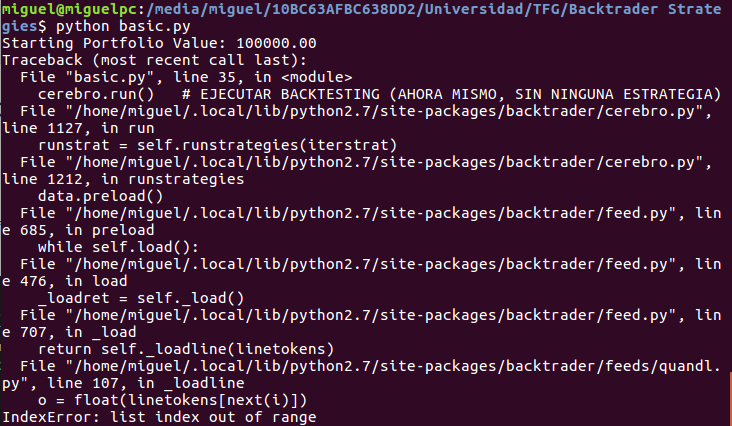
\includegraphics[scale=1.2]{imagenes/quandl_install.png}
				\caption{Ejecuci\'on del script recolectando datos de Quandl.}
				\label{fig:quandl_install}
			\end{figure}
			
			
		\subsection{YAHOO! Finance}
				
		Una de las opciones m\'as completas para conseguir los datos es la p\'agina web de YAHOO! Finance (\url{https://finance.yahoo.com}). Basta con buscar el \'indice o la empresa sobre la que se quieren los datos, indicar las fechas y la frecuencia de muestreo y pinchar en el bot\'on de descarga. Los datos se descargan en formato CSV. Este formato es ampliamente utilizado por la comunidad cient\'ifica para almacenar grandes cantidades de datos.\\
				
		\begin{figure}[H]
			\centering
			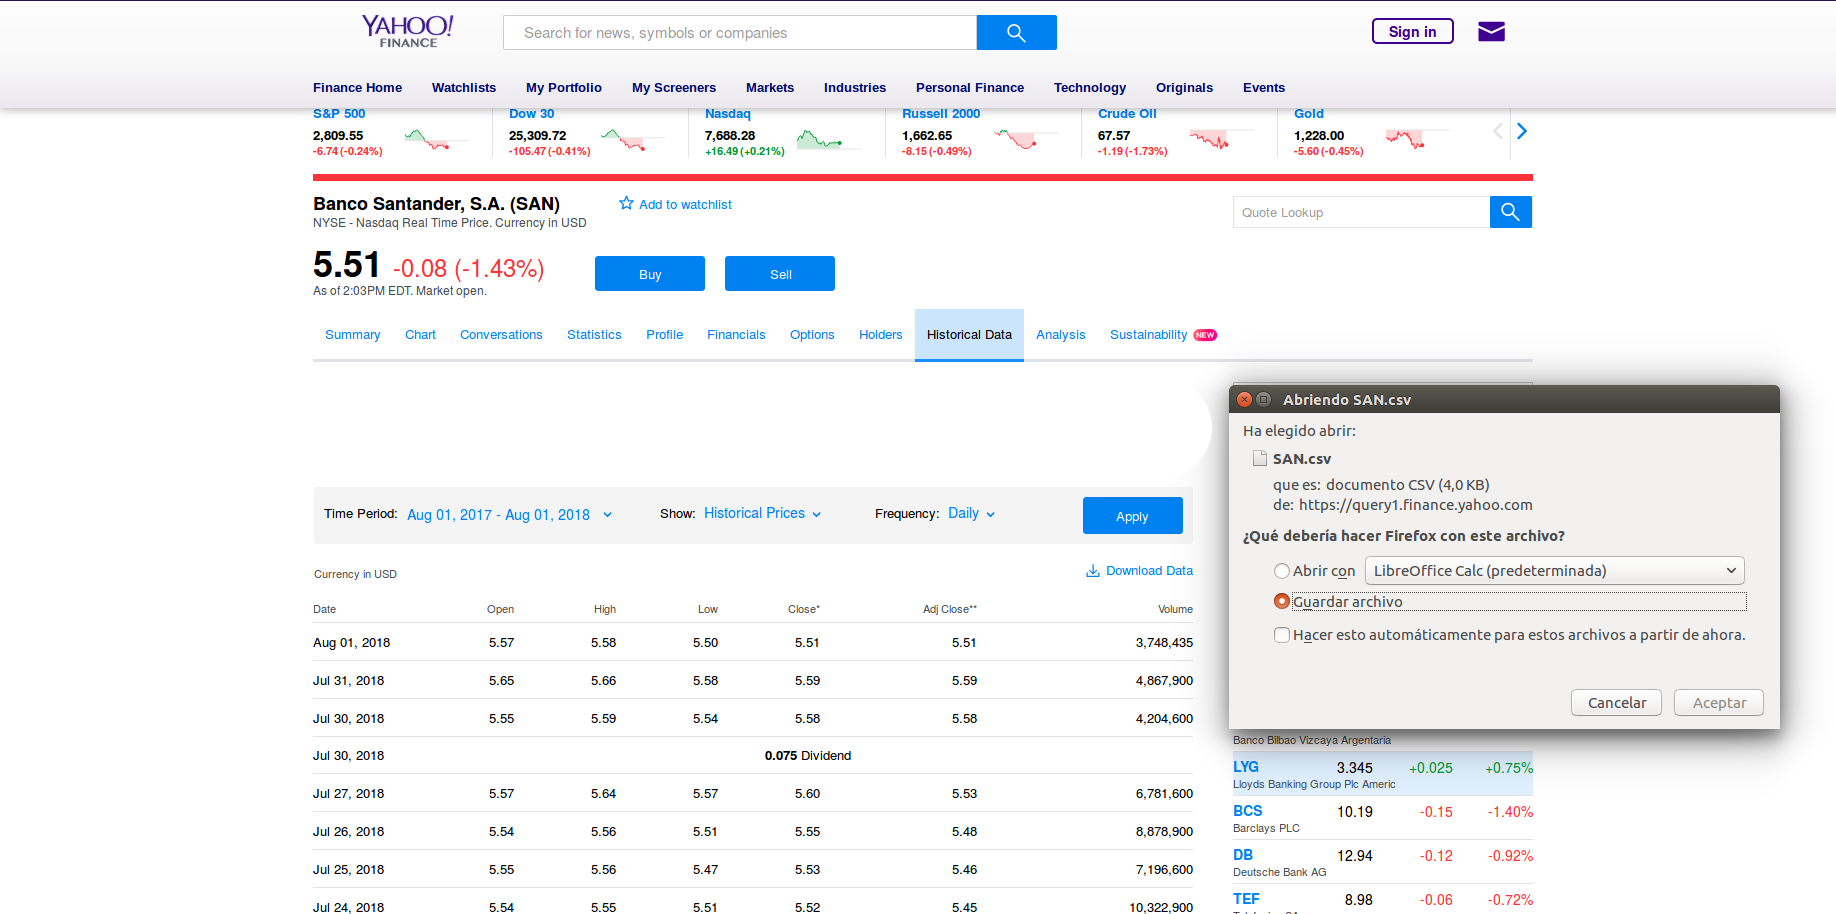
\includegraphics[scale=1]{imagenes/yahoo_finance.png}
			\caption{Descarga de los datos hist\'oricos de Banco Santander.}
			\label{fig:yahoo_finance}
		\end{figure}
				
		Por ejemplo, imaginemos que buscamos los valores hist\'oricos de Banco Santander desde el 1 de agosto de 2017 hasta la misma fecha del a\~{n}o siguiente. Para ello indicamos la empresa, nos vamos al apartado de \textit{Historical Data} e indicamos las fechas. El resultado se muestra en la figura \ref{fig:yahoo_finance}.\\
		
		Para cargar estos datos en backtrader basta con indicar la ruta y el rango de fechas con el siguiente c\'odigo:

		\begin{lstlisting}[basicstyle=\tiny]
   # Crear un paquete de datos con YAHOO FINANCE
   data = bt.feeds.YahooFinanceCSVData(
	   dataname='Data/SAN.csv',
	   fromdate=datetime.datetime(2017, 8, 1),
	   todate=datetime.datetime(2018, 8, 1),
	   reverse=False)
   
   # Activar los datos en el cerebro
   cerebro.adddata(data)
		\end{lstlisting}		
		
	\newpage	
	\section{Algor\'itmos gen\'eticos}
	
		\subsection{Definici\'on}
			\subsubsection{Poblaci\'on}
			\subsubsection{Funci\'on fitness}
			\subsubsection{Cruce}
			\subsubsection{Mutaci\'on}
		\subsection{Pyvolution}
		
		Pyvolution es un paquete de Python de algoritmos gen\'eticos. Aunque la \'ultima versi\'on fue lanzada en 2012, es un paquete completo y sencillo de utilizar. En apenas 30 lineas y sin necesidad de dar muchas especificaciones se pueden realizar algoritmos completos. Una ejecuci\'on normal consta de varios par\'ametros donde se pueden controlar las generaciones, los individuos por generaci\'on, probabilidad y severidad de las mutaciones, cantidad indiviudos elitistas e incluso el tiempo m\'aximo de ejecuci\'on.\\
		
		Para ilustrar brevemente su uso, muestro uno de los ejemplos que vienen en la p\'agina de Github del paquete.
		
		\begin{lstlisting}[basicstyle=\tiny]
	import math
	from pyvolution.EvolutionManager import *
	from pyvolution.GeneLibrary import *
	
	"""
	Queremos calcular una solucion del siguiente sistema:
	a + b + c - 17 = 0
	a^2 + b^2 - 5 = 0
	"""
		
	def fitnessFunction(chromosome):
		"""
		Dado un "cromosoma", esta es la funcion que calcula su puntuacion
		La puntuacion es una float mayor que 0.
		"""
		
		#Accedemos a los cromosomas o valores a ajustar
		a = chromosome["a"]
		b = chromosome["b"]
		c = chromosome["c"]
		d = chromosome["d"]
		
		#Calculamos los valores que nos gustaria que fueran 0
		val1 = math.fabs(a + b + c - 17)
		val2 = math.fabs(math.pow(a, 2) + math.pow(b, 2) - 5)
		
		#La funcion distancia agrupa los valores para una mejor puntuacion
		dist = math.sqrt(math.pow(val1, 2) + math.pow(val2, 2)
		
		if dist != 0:
		return 1 / dist # Cuanto menor sea la distancia mayor sera la puntuacion
		else:
		return None     #Devolver None indica que los cromosomas han sido ajustados
		
		
	#Configuramos el algoritmo genetico
	em = EvolutionManager(
		fitnessFunction,
		individualsPerGeneration=100,
		mutationRate=0.2,	#Probabilidad de mutacion
		maxGenerations=1000,
		stopAfterTime=10,   #Para simulacion tras 10 segundos
		elitism=2,          #Mantener los 2 mejores de cada generacion
	)
		
	#Creamos una funcion de mutacion inversamente proporcional a la bondad del ajuste
	mutator = FloatInverseFit("mut", maxVal=0.01, startVal=1)
		
	#Indicamos que los puntos iniciales se toman siguiendo una distribucion normal
	#de media 0 y desviacion 100. Ademas marcamos la mutacion como la definida antes.
	atype = FloatGeneType("a", generatorAverage=0, generatorSTDEV=100, mutatorGene="mut")
	btype = FloatGeneType("b", generatorAverage=0, generatorSTDEV=100, mutatorGene="mut")
	ctype = FloatGeneType("c", generatorAverage=0, generatorSTDEV=100, mutatorGene="mut")
		
	#Registramos los parametos y la mutacion
	em.addGeneType(mutator)
	em.addGeneType(atype)
	em.addGeneType(btype)
	em.addGeneType(ctype)
	
	#Ejecutamos	
	result = em.run()
		\end{lstlisting}
	
	\newpage
	\section{\'Arbol de Decisi\'on}\label{sec:Decision_tree}
	
		Los \'arboles se utilizan en diversos campos de la inform\'atica y, en concreto, en la toma de decisiones y/o predicciones. A pesar de que son dif\'iciles de representar y visualizar de forma global, resultan una herramienta muy \'util para separar situaciones o datos seg\'un una serie de condiciones dadas previamente.
		
		\subsection{Definici\'on}
			Un grafo simple es un grafo sin lazos ni aristas m\'ultiples entre sus v\'ertices. Un \'arbol es un grafo simple G tal que
			para cada dos v\'ertices de G existe un \'unico camino simple entre ellos.
			
			Un \'arbol de decisi\'on ser\'a, por tanto, un \'arbol compuesto por:
			\begin{itemize}
				\item Un v\'ertice especial, llamado nodo ra\'iz, que se considera el inicio del camino de decisi\'on.
				\item Un conjunto de v\'ertices, llamados nodos, conectados con al menos otros 2 v\'ertices. En cada nodo hay una condici\'on. La verficaci\'on de dicha condici\'on determina que nodo es el siguiente en el camino de decisi\'on.
				\item Un conjunto de v\'ertices, llamados hojas o nodos terminales, conectados con un \'unico v\'ertice. En cada hoja hay una decisi\'on que deber\'ia ser tomada si el camino de decisi\'on lleva hasta \'el.
			\end{itemize}
			\subsubsection{Etiquetado}
			\subsubsection{Generaci\'on de un \'arbol}
			\subsubsection{Sobreaprendizaje}
	
	
	
		
\newpage

\bibliographystyle{plain}
\bibliography{bibliografia.bib}

\end{document}
